\documentclass[twoside]{book}

% Packages required by doxygen
\usepackage{fixltx2e}
\usepackage{calc}
\usepackage{doxygen}
\usepackage[export]{adjustbox} % also loads graphicx
\usepackage{graphicx}
\usepackage[utf8]{inputenc}
\usepackage{makeidx}
\usepackage{multicol}
\usepackage{multirow}
\PassOptionsToPackage{warn}{textcomp}
\usepackage{textcomp}
\usepackage[nointegrals]{wasysym}
\usepackage[table]{xcolor}

% Font selection
\usepackage[T1]{fontenc}
\usepackage[scaled=.90]{helvet}
\usepackage{courier}
\usepackage{amssymb}
\usepackage{sectsty}
\renewcommand{\familydefault}{\sfdefault}
\allsectionsfont{%
  \fontseries{bc}\selectfont%
  \color{darkgray}%
}
\renewcommand{\DoxyLabelFont}{%
  \fontseries{bc}\selectfont%
  \color{darkgray}%
}
\newcommand{\+}{\discretionary{\mbox{\scriptsize$\hookleftarrow$}}{}{}}

% Page & text layout
\usepackage{geometry}
\geometry{%
  a4paper,%
  top=2.5cm,%
  bottom=2.5cm,%
  left=2.5cm,%
  right=2.5cm%
}
\tolerance=750
\hfuzz=15pt
\hbadness=750
\setlength{\emergencystretch}{15pt}
\setlength{\parindent}{0cm}
\setlength{\parskip}{3ex plus 2ex minus 2ex}
\makeatletter
\renewcommand{\paragraph}{%
  \@startsection{paragraph}{4}{0ex}{-1.0ex}{1.0ex}{%
    \normalfont\normalsize\bfseries\SS@parafont%
  }%
}
\renewcommand{\subparagraph}{%
  \@startsection{subparagraph}{5}{0ex}{-1.0ex}{1.0ex}{%
    \normalfont\normalsize\bfseries\SS@subparafont%
  }%
}
\makeatother

% Headers & footers
\usepackage{fancyhdr}
\pagestyle{fancyplain}
\fancyhead[LE]{\fancyplain{}{\bfseries\thepage}}
\fancyhead[CE]{\fancyplain{}{}}
\fancyhead[RE]{\fancyplain{}{\bfseries\leftmark}}
\fancyhead[LO]{\fancyplain{}{\bfseries\rightmark}}
\fancyhead[CO]{\fancyplain{}{}}
\fancyhead[RO]{\fancyplain{}{\bfseries\thepage}}
\fancyfoot[LE]{\fancyplain{}{}}
\fancyfoot[CE]{\fancyplain{}{}}
\fancyfoot[RE]{\fancyplain{}{\bfseries\scriptsize Generated by Doxygen }}
\fancyfoot[LO]{\fancyplain{}{\bfseries\scriptsize Generated by Doxygen }}
\fancyfoot[CO]{\fancyplain{}{}}
\fancyfoot[RO]{\fancyplain{}{}}
\renewcommand{\footrulewidth}{0.4pt}
\renewcommand{\chaptermark}[1]{%
  \markboth{#1}{}%
}
\renewcommand{\sectionmark}[1]{%
  \markright{\thesection\ #1}%
}

% Indices & bibliography
\usepackage{natbib}
\usepackage[titles]{tocloft}
\setcounter{tocdepth}{3}
\setcounter{secnumdepth}{5}
\makeindex

% Hyperlinks (required, but should be loaded last)
\usepackage{ifpdf}
\ifpdf
  \usepackage[pdftex,pagebackref=true]{hyperref}
\else
  \usepackage[ps2pdf,pagebackref=true]{hyperref}
\fi
\hypersetup{%
  colorlinks=true,%
  linkcolor=blue,%
  citecolor=blue,%
  unicode%
}

% Custom commands
\newcommand{\clearemptydoublepage}{%
  \newpage{\pagestyle{empty}\cleardoublepage}%
}

\usepackage{caption}
\captionsetup{labelsep=space,justification=centering,font={bf},singlelinecheck=off,skip=4pt,position=top}

%===== C O N T E N T S =====

\begin{document}

% Titlepage & ToC
\hypersetup{pageanchor=false,
             bookmarksnumbered=true,
             pdfencoding=unicode
            }
\pagenumbering{alph}
\begin{titlepage}
\vspace*{7cm}
\begin{center}%
{\Large My Project }\\
\vspace*{1cm}
{\large Generated by Doxygen 1.8.13}\\
\end{center}
\end{titlepage}
\clearemptydoublepage
\pagenumbering{roman}
\tableofcontents
\clearemptydoublepage
\pagenumbering{arabic}
\hypersetup{pageanchor=true}

%--- Begin generated contents ---
\chapter{Hierarchical Index}
\section{Class Hierarchy}
This inheritance list is sorted roughly, but not completely, alphabetically\+:\begin{DoxyCompactList}
\item \contentsline{section}{twitter.\+views.\+Twitter\+Stats}{\pageref{classtwitter_1_1views_1_1_twitter_stats}}{}
\item App\+Config\begin{DoxyCompactList}
\item \contentsline{section}{twitter.\+apps.\+Twitter\+Config}{\pageref{classtwitter_1_1apps_1_1_twitter_config}}{}
\end{DoxyCompactList}
\item Test\+Case\begin{DoxyCompactList}
\item \contentsline{section}{twitter.\+tests.\+Stats\+Test\+Cases}{\pageref{classtwitter_1_1tests_1_1_stats_test_cases}}{}
\end{DoxyCompactList}
\end{DoxyCompactList}

\chapter{Class Index}
\section{Class List}
Here are the classes, structs, unions and interfaces with brief descriptions\+:\begin{DoxyCompactList}
\item\contentsline{section}{\hyperlink{classtwitter_1_1tests_1_1_stats_test_cases}{twitter.\+tests.\+Stats\+Test\+Cases} }{\pageref{classtwitter_1_1tests_1_1_stats_test_cases}}{}
\item\contentsline{section}{\hyperlink{classtwitter_1_1apps_1_1_twitter_config}{twitter.\+apps.\+Twitter\+Config} }{\pageref{classtwitter_1_1apps_1_1_twitter_config}}{}
\item\contentsline{section}{\hyperlink{classtwitter_1_1views_1_1_twitter_stats}{twitter.\+views.\+Twitter\+Stats} }{\pageref{classtwitter_1_1views_1_1_twitter_stats}}{}
\end{DoxyCompactList}

\chapter{Class Documentation}
\hypertarget{classtwitter_1_1tests_1_1_stats_test_cases}{}\section{twitter.\+tests.\+Stats\+Test\+Cases Class Reference}
\label{classtwitter_1_1tests_1_1_stats_test_cases}\index{twitter.\+tests.\+Stats\+Test\+Cases@{twitter.\+tests.\+Stats\+Test\+Cases}}
Inheritance diagram for twitter.\+tests.\+Stats\+Test\+Cases\+:\begin{figure}[H]
\begin{center}
\leavevmode
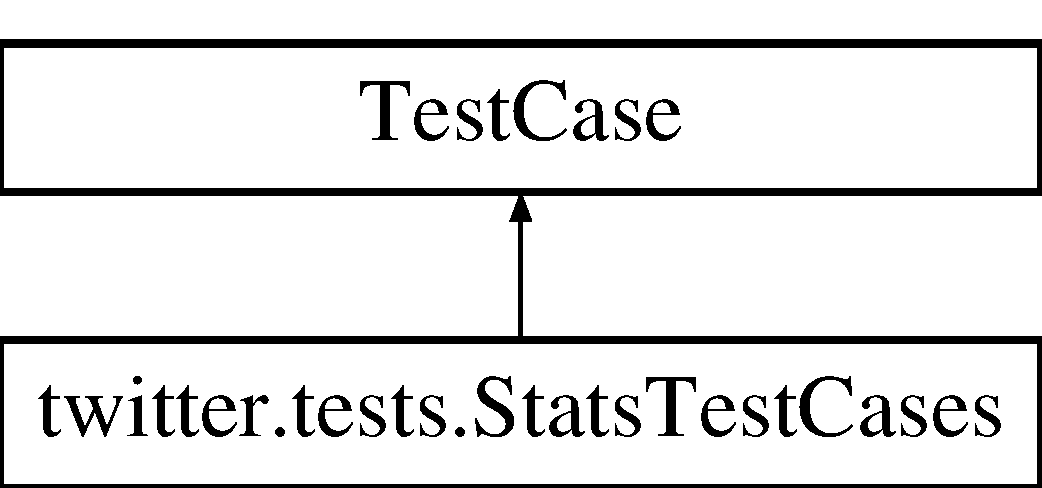
\includegraphics[height=2.000000cm]{classtwitter_1_1tests_1_1_stats_test_cases}
\end{center}
\end{figure}
\subsection*{Public Member Functions}
\begin{DoxyCompactItemize}
\item 
\mbox{\Hypertarget{classtwitter_1_1tests_1_1_stats_test_cases_ae7e663218f193abe62a2ec355bcd976e}\label{classtwitter_1_1tests_1_1_stats_test_cases_ae7e663218f193abe62a2ec355bcd976e}} 
def {\bfseries test\+\_\+get\+Frequency\+Of\+Words\+Of\+Liked\+Tweets} (self)
\item 
\mbox{\Hypertarget{classtwitter_1_1tests_1_1_stats_test_cases_aab32d136d9438b12de98a3f691946432}\label{classtwitter_1_1tests_1_1_stats_test_cases_aab32d136d9438b12de98a3f691946432}} 
def {\bfseries test\+\_\+who\+Mentioned\+Most} (self)
\item 
\mbox{\Hypertarget{classtwitter_1_1tests_1_1_stats_test_cases_a78a25891e8faaa226a38a43539ecb5a9}\label{classtwitter_1_1tests_1_1_stats_test_cases_a78a25891e8faaa226a38a43539ecb5a9}} 
def {\bfseries test\+\_\+get\+Most\+Liked\+Pages} (self)
\item 
\mbox{\Hypertarget{classtwitter_1_1tests_1_1_stats_test_cases_ab61ba217f8dfe8a84e7d33de828bdaf2}\label{classtwitter_1_1tests_1_1_stats_test_cases_ab61ba217f8dfe8a84e7d33de828bdaf2}} 
def {\bfseries test\+\_\+get\+Users\+Tweeting\+Most\+Frequently} (self)
\item 
\mbox{\Hypertarget{classtwitter_1_1tests_1_1_stats_test_cases_a3581f04cb8a74b0559e63ed8caccce4d}\label{classtwitter_1_1tests_1_1_stats_test_cases_a3581f04cb8a74b0559e63ed8caccce4d}} 
def {\bfseries test\+\_\+get\+Frequency\+Of\+Words\+Of\+All\+Tweets} (self)
\item 
\mbox{\Hypertarget{classtwitter_1_1tests_1_1_stats_test_cases_a2379f24f8f9c91e49709bc01e8d32637}\label{classtwitter_1_1tests_1_1_stats_test_cases_a2379f24f8f9c91e49709bc01e8d32637}} 
def {\bfseries test\+\_\+get\+Like\+Ratio\+Of\+Two\+Users} (self)
\item 
\mbox{\Hypertarget{classtwitter_1_1tests_1_1_stats_test_cases_ae2af08fbd0d5c8d92b1e8f5d0a183ede}\label{classtwitter_1_1tests_1_1_stats_test_cases_ae2af08fbd0d5c8d92b1e8f5d0a183ede}} 
def {\bfseries test\+\_\+get\+Hashtag\+Percentage} (self)
\item 
\mbox{\Hypertarget{classtwitter_1_1tests_1_1_stats_test_cases_af724a16f2c313472fb69dc39e727c23b}\label{classtwitter_1_1tests_1_1_stats_test_cases_af724a16f2c313472fb69dc39e727c23b}} 
def {\bfseries test\+\_\+get\+Most\+Number\+Of\+Followers} (self)
\end{DoxyCompactItemize}


The documentation for this class was generated from the following file\+:\begin{DoxyCompactItemize}
\item 
tests.\+py\end{DoxyCompactItemize}

\hypertarget{classtwitter_1_1apps_1_1_twitter_config}{}\section{twitter.\+apps.\+Twitter\+Config Class Reference}
\label{classtwitter_1_1apps_1_1_twitter_config}\index{twitter.\+apps.\+Twitter\+Config@{twitter.\+apps.\+Twitter\+Config}}
Inheritance diagram for twitter.\+apps.\+Twitter\+Config\+:\begin{figure}[H]
\begin{center}
\leavevmode
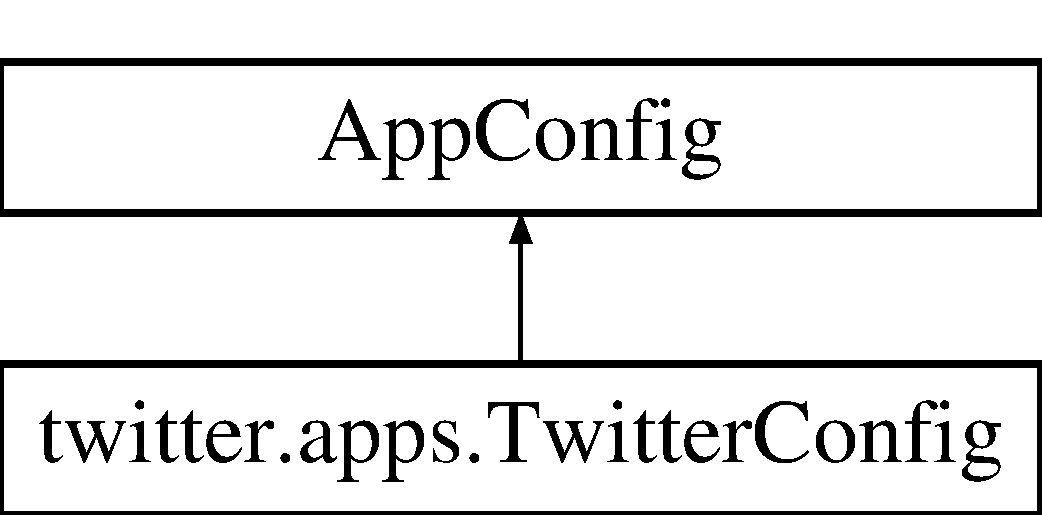
\includegraphics[height=2.000000cm]{classtwitter_1_1apps_1_1_twitter_config}
\end{center}
\end{figure}
\subsection*{Static Public Attributes}
\begin{DoxyCompactItemize}
\item 
\mbox{\Hypertarget{classtwitter_1_1apps_1_1_twitter_config_ad6fa8da3b1d7a28a13a3a1430d9ad93f}\label{classtwitter_1_1apps_1_1_twitter_config_ad6fa8da3b1d7a28a13a3a1430d9ad93f}} 
string {\bfseries name} = \textquotesingle{}twitter\textquotesingle{}
\end{DoxyCompactItemize}


The documentation for this class was generated from the following file\+:\begin{DoxyCompactItemize}
\item 
apps.\+py\end{DoxyCompactItemize}

\hypertarget{classtwitter_1_1views_1_1_twitter_stats}{}\section{twitter.\+views.\+Twitter\+Stats Class Reference}
\label{classtwitter_1_1views_1_1_twitter_stats}\index{twitter.\+views.\+Twitter\+Stats@{twitter.\+views.\+Twitter\+Stats}}
\subsection*{Public Member Functions}
\begin{DoxyCompactItemize}
\item 
\mbox{\Hypertarget{classtwitter_1_1views_1_1_twitter_stats_ae34b27b044e8f8493952f856866e1528}\label{classtwitter_1_1views_1_1_twitter_stats_ae34b27b044e8f8493952f856866e1528}} 
def {\bfseries index} (request)
\item 
\mbox{\Hypertarget{classtwitter_1_1views_1_1_twitter_stats_af34b050b301a95d439181f762ec5448f}\label{classtwitter_1_1views_1_1_twitter_stats_af34b050b301a95d439181f762ec5448f}} 
def {\bfseries example} (request)
\item 
def \hyperlink{classtwitter_1_1views_1_1_twitter_stats_a1b25912ecee8b0ee19af0948378a57fa}{get\+Users\+Tweeting\+Most\+Frequently} (request)
\item 
def \hyperlink{classtwitter_1_1views_1_1_twitter_stats_a880c4da522b5f91c401c54861dc3ad12}{get\+Frequency\+Of\+Words\+Of\+Liked\+Tweets} (request)
\item 
\mbox{\Hypertarget{classtwitter_1_1views_1_1_twitter_stats_aab4275f1224264499ea247a721fa23ce}\label{classtwitter_1_1views_1_1_twitter_stats_aab4275f1224264499ea247a721fa23ce}} 
def {\bfseries get\+Most\+Number\+Of\+Followers} (request)
\item 
\mbox{\Hypertarget{classtwitter_1_1views_1_1_twitter_stats_ae955472d98f39a044a91efef95b7b156}\label{classtwitter_1_1views_1_1_twitter_stats_ae955472d98f39a044a91efef95b7b156}} 
def {\bfseries get\+Most\+Liked\+Pages} (request)
\item 
def \hyperlink{classtwitter_1_1views_1_1_twitter_stats_a45827ee187a326fb1394d680bc483fb9}{get\+Who\+Mentioned\+Most} (request)
\item 
def \hyperlink{classtwitter_1_1views_1_1_twitter_stats_a48eab8e241bb382791c9f2803b57ca34}{get\+Frequency\+Of\+Words\+Of\+All\+Tweets} (request)
\item 
def \hyperlink{classtwitter_1_1views_1_1_twitter_stats_ae06146619068fb60465d6f99c4f9c369}{get\+Like\+Ratio\+Of\+Two\+Users} (request)
\item 
\mbox{\Hypertarget{classtwitter_1_1views_1_1_twitter_stats_a78a796f6ed9c85bd1b8d5614138b84e6}\label{classtwitter_1_1views_1_1_twitter_stats_a78a796f6ed9c85bd1b8d5614138b84e6}} 
def {\bfseries hashtag\+Percentage} (request)
\end{DoxyCompactItemize}
\subsection*{Static Public Member Functions}
\begin{DoxyCompactItemize}
\item 
\mbox{\Hypertarget{classtwitter_1_1views_1_1_twitter_stats_aa259d1356864ab08580a065ea7228ab6}\label{classtwitter_1_1views_1_1_twitter_stats_aa259d1356864ab08580a065ea7228ab6}} 
def {\bfseries get\+Twitter\+Api} ()
\end{DoxyCompactItemize}


\subsection{Member Function Documentation}
\mbox{\Hypertarget{classtwitter_1_1views_1_1_twitter_stats_a48eab8e241bb382791c9f2803b57ca34}\label{classtwitter_1_1views_1_1_twitter_stats_a48eab8e241bb382791c9f2803b57ca34}} 
\index{twitter\+::views\+::\+Twitter\+Stats@{twitter\+::views\+::\+Twitter\+Stats}!get\+Frequency\+Of\+Words\+Of\+All\+Tweets@{get\+Frequency\+Of\+Words\+Of\+All\+Tweets}}
\index{get\+Frequency\+Of\+Words\+Of\+All\+Tweets@{get\+Frequency\+Of\+Words\+Of\+All\+Tweets}!twitter\+::views\+::\+Twitter\+Stats@{twitter\+::views\+::\+Twitter\+Stats}}
\subsubsection{\texorpdfstring{get\+Frequency\+Of\+Words\+Of\+All\+Tweets()}{getFrequencyOfWordsOfAllTweets()}}
{\footnotesize\ttfamily def twitter.\+views.\+Twitter\+Stats.\+get\+Frequency\+Of\+Words\+Of\+All\+Tweets (\begin{DoxyParamCaption}\item[{}]{request }\end{DoxyParamCaption})}

\begin{DoxyVerb}This method counts the frequency of the words a specific user own tweets.
It has two paramters, username and count where username is compulsory.
If a username is not provided, method returns a string that expresses this fact.
If count is not provided, it is defaulted to 1, hence only 1 tweets is searched.

author: Fatih Asagidag
\end{DoxyVerb}
 \mbox{\Hypertarget{classtwitter_1_1views_1_1_twitter_stats_a880c4da522b5f91c401c54861dc3ad12}\label{classtwitter_1_1views_1_1_twitter_stats_a880c4da522b5f91c401c54861dc3ad12}} 
\index{twitter\+::views\+::\+Twitter\+Stats@{twitter\+::views\+::\+Twitter\+Stats}!get\+Frequency\+Of\+Words\+Of\+Liked\+Tweets@{get\+Frequency\+Of\+Words\+Of\+Liked\+Tweets}}
\index{get\+Frequency\+Of\+Words\+Of\+Liked\+Tweets@{get\+Frequency\+Of\+Words\+Of\+Liked\+Tweets}!twitter\+::views\+::\+Twitter\+Stats@{twitter\+::views\+::\+Twitter\+Stats}}
\subsubsection{\texorpdfstring{get\+Frequency\+Of\+Words\+Of\+Liked\+Tweets()}{getFrequencyOfWordsOfLikedTweets()}}
{\footnotesize\ttfamily def twitter.\+views.\+Twitter\+Stats.\+get\+Frequency\+Of\+Words\+Of\+Liked\+Tweets (\begin{DoxyParamCaption}\item[{}]{request }\end{DoxyParamCaption})}

\begin{DoxyVerb}This method counts the frequency of the words a specific user liked.
It has two paramters, username and count where username is compulsory.
If a username is not provided, method returns a string that expresses this fact.
If count is not provided, it is defaulted to 100, hence only 100 tweets is searched.

author: Riza Ozcelik
\end{DoxyVerb}
 \mbox{\Hypertarget{classtwitter_1_1views_1_1_twitter_stats_ae06146619068fb60465d6f99c4f9c369}\label{classtwitter_1_1views_1_1_twitter_stats_ae06146619068fb60465d6f99c4f9c369}} 
\index{twitter\+::views\+::\+Twitter\+Stats@{twitter\+::views\+::\+Twitter\+Stats}!get\+Like\+Ratio\+Of\+Two\+Users@{get\+Like\+Ratio\+Of\+Two\+Users}}
\index{get\+Like\+Ratio\+Of\+Two\+Users@{get\+Like\+Ratio\+Of\+Two\+Users}!twitter\+::views\+::\+Twitter\+Stats@{twitter\+::views\+::\+Twitter\+Stats}}
\subsubsection{\texorpdfstring{get\+Like\+Ratio\+Of\+Two\+Users()}{getLikeRatioOfTwoUsers()}}
{\footnotesize\ttfamily def twitter.\+views.\+Twitter\+Stats.\+get\+Like\+Ratio\+Of\+Two\+Users (\begin{DoxyParamCaption}\item[{}]{request }\end{DoxyParamCaption})}

\begin{DoxyVerb}This method takes two usernames and finds the like counts of each others' posts.
Returns 'MISSING USERNAME' when at least one username is not provided.
100 tweets are taken from timeline for both users.

author: Hilal Benzer
\end{DoxyVerb}
 \mbox{\Hypertarget{classtwitter_1_1views_1_1_twitter_stats_a1b25912ecee8b0ee19af0948378a57fa}\label{classtwitter_1_1views_1_1_twitter_stats_a1b25912ecee8b0ee19af0948378a57fa}} 
\index{twitter\+::views\+::\+Twitter\+Stats@{twitter\+::views\+::\+Twitter\+Stats}!get\+Users\+Tweeting\+Most\+Frequently@{get\+Users\+Tweeting\+Most\+Frequently}}
\index{get\+Users\+Tweeting\+Most\+Frequently@{get\+Users\+Tweeting\+Most\+Frequently}!twitter\+::views\+::\+Twitter\+Stats@{twitter\+::views\+::\+Twitter\+Stats}}
\subsubsection{\texorpdfstring{get\+Users\+Tweeting\+Most\+Frequently()}{getUsersTweetingMostFrequently()}}
{\footnotesize\ttfamily def twitter.\+views.\+Twitter\+Stats.\+get\+Users\+Tweeting\+Most\+Frequently (\begin{DoxyParamCaption}\item[{}]{request }\end{DoxyParamCaption})}

\begin{DoxyVerb}This method finds users who has been tweeting most frequently (on hourly basis).
It checks for the time difference between request and tweets.
The tweets are collected from timeline.

author: Anil Seyrek
\end{DoxyVerb}
 \mbox{\Hypertarget{classtwitter_1_1views_1_1_twitter_stats_a45827ee187a326fb1394d680bc483fb9}\label{classtwitter_1_1views_1_1_twitter_stats_a45827ee187a326fb1394d680bc483fb9}} 
\index{twitter\+::views\+::\+Twitter\+Stats@{twitter\+::views\+::\+Twitter\+Stats}!get\+Who\+Mentioned\+Most@{get\+Who\+Mentioned\+Most}}
\index{get\+Who\+Mentioned\+Most@{get\+Who\+Mentioned\+Most}!twitter\+::views\+::\+Twitter\+Stats@{twitter\+::views\+::\+Twitter\+Stats}}
\subsubsection{\texorpdfstring{get\+Who\+Mentioned\+Most()}{getWhoMentionedMost()}}
{\footnotesize\ttfamily def twitter.\+views.\+Twitter\+Stats.\+get\+Who\+Mentioned\+Most (\begin{DoxyParamCaption}\item[{}]{request }\end{DoxyParamCaption})}

\begin{DoxyVerb}author: Ezgi Yuceturk
This method to find the follower who has recently been mentioned most by the authenticated user the most.
\end{DoxyVerb}
 

The documentation for this class was generated from the following file\+:\begin{DoxyCompactItemize}
\item 
views.\+py\end{DoxyCompactItemize}

%--- End generated contents ---

% Index
\backmatter
\newpage
\phantomsection
\clearemptydoublepage
\addcontentsline{toc}{chapter}{Index}
\printindex

\end{document}
